\FloatBarrier

Nur die elektromagnetische Wechselwirkung ist von Bedeutung. Folgende Reaktionen führen zu einem
Energieverlust von geladenen Teilchen in Materie:

\begin{itemize}
  \item Ionisation der Atome im Detektormaterial
  \item Anregung der Atome im Detektormaterial
  \item Bremsstrahlung (relevant für Elektronen/Positronen)
  \item \v{C}erenkov-Strahlung
  \item Übergangsstrahlung
\end{itemize}
 
 Beispiel: Gesamte Energieverlustrate $-\frac{\mathrm{d}E}{\mathrm{d}x}$ für Myonen in Kupfer (s. Abb.
 \ref{myonenInKupfer)}). Der Großteil wird durch die Bethe-Bloch-Formel beschrieben (Herleitung
 erfolgt im nächsten Kapitel).
Unterschiedliche Energie der Projektile führt über unterschiedliche Wechselwirkung zum
Energieverlust.

\begin{align*}
-\left(\frac{\mathrm{d}E}{\mathrm{d}x}\right)_{\text{tot}} &= -\left(\frac{\mathrm{d}E}{\mathrm{d}x}\right)_{\text{coll}}
-\left(\frac{\mathrm{d}E}{\mathrm{d}x}\right)_{\text{rad}} -\left(\frac{\mathrm{d}E}{\mathrm{d}x}\right)_{\text{pair}}
-\left(\frac{\mathrm{d}E}{\mathrm{d}x}\right)_{\text{photo}} -\left(\frac{\mathrm{d}E}{\mathrm{d}x}\right)_{\text{compt}} \\
&\hspace{4mm} -\left(\frac{\mathrm{d}E}{\mathrm{d}x}\right)_{\text{kal}}-\ldots
\end{align*}
 
\begin{figure}
	\centering
	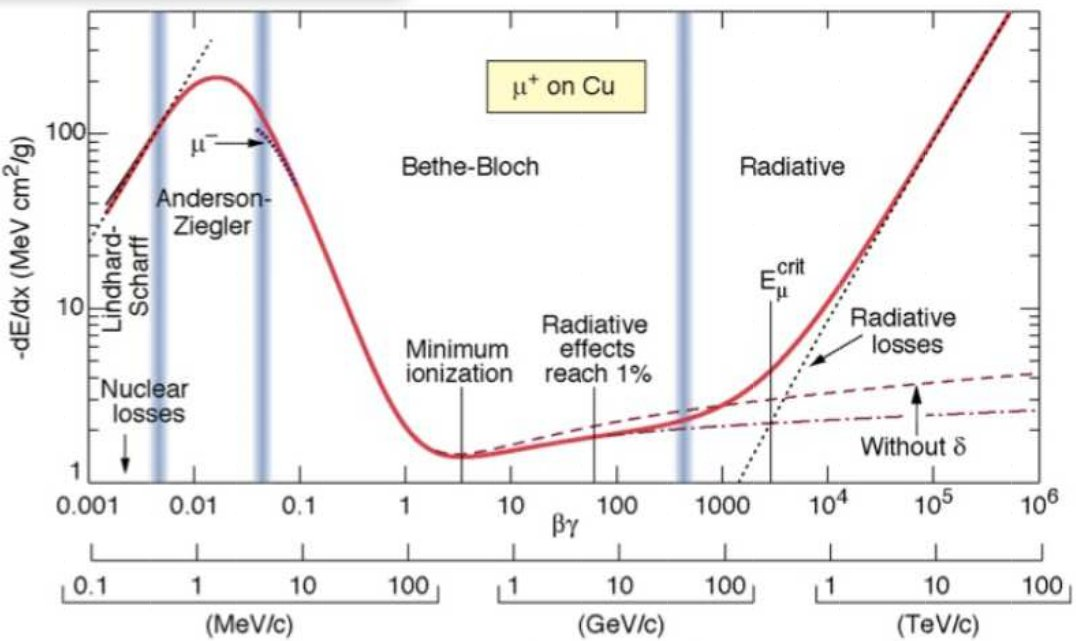
\includegraphics[width=0.5\textwidth]{bethebloch.jpg}
 	\caption{Energieverlust von Myonen in Kupfer}
 	\label{myonenInKupfer}
\end{figure}

\begin{figure}
	\centering
	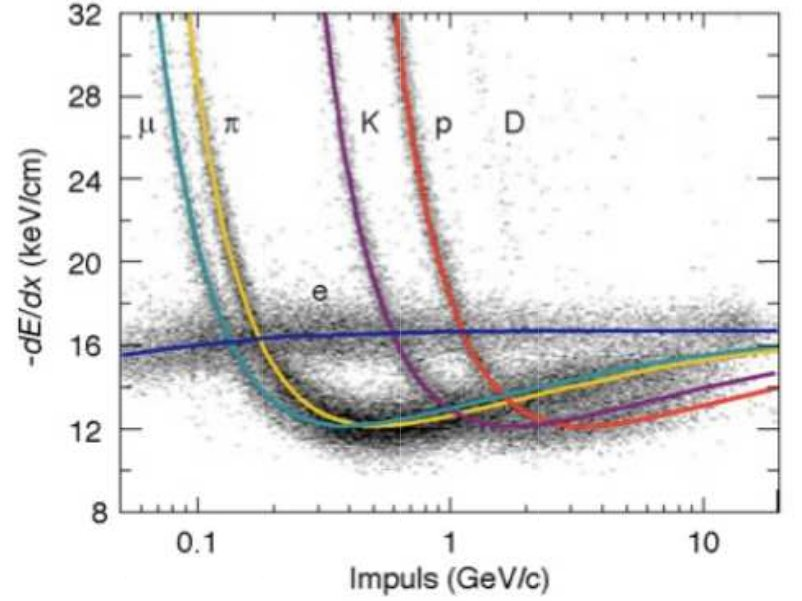
\includegraphics[width=0.5\textwidth]{bethebloch2.jpg}
	\caption{$\frac{\mathrm{d}E}{\mathrm{d}x}$-Kurven für verschiedene Teilchen (gemessen in der
	PEP4/9-TPC)}
	\label{}
\end{figure}
 
 Beachte: $\frac{\mathrm{d}E}{\mathrm{d}x}$ für "`schwere"' Teilchen (z.B. $\alpha$) wird in diesem Impulsbereich gut
 durch die Bethe-Bloch-Formel beschrieben. Der Energieverlust durch Ionisation und Anregung von
 Targetelektronen dominiert. $\frac{\mathrm{d}E}{\mathrm{d}x}$ für Elektronen/Positronen folgt jedoch nicht der
 Bethe-Bloch-Formel!
 
 \FloatBarrier